\chapter{Data Augmentation for Satellite Imagery}
\label{ch:aug}

\chapmeta{Intermediate}{$\sim$4\,h (1.5\,h + 2.5\,h)}{EuroSAT; LoveDA}

\begin{objbox}
\begin{itemize}[leftmargin=1.2em,nosep]
  \item Build geometric and photometric augmentation pipelines with \texttt{albumentations}.
  \item Identify which augmentations are label-safe for satellite imagery and which are not.
  \item Apply joint image+mask augmentation for segmentation.
  \item Understand and implement MixUp and CutMix.
  \item Empirically measure the accuracy gain from augmentation via an ablation.
\end{itemize}
\end{objbox}

Augmentation is the cheapest and most reliable regulariser for vision models: it
synthesises new, label-consistent training examples on the fly, expanding the
effective dataset and encoding invariances we know the task should have.
Satellite imagery has a special property that makes some augmentations
\emph{more} valid than for natural photos --- and others invalid.

\section{Why augmentation is especially powerful in EO}

Nadir-looking satellite scenes have no canonical ``up''. A forest rotated 90°
or mirrored is still a forest, so the full dihedral group of flips and
90°-rotations is label-preserving --- eight free views of every patch, an
invariance natural photos do not enjoy. Combined with the chronic scarcity of
labels in EO, this makes geometric augmentation unusually effective.
Figure~\ref{fig:aug} shows representative transforms.

\begin{figure}[h]
\centering
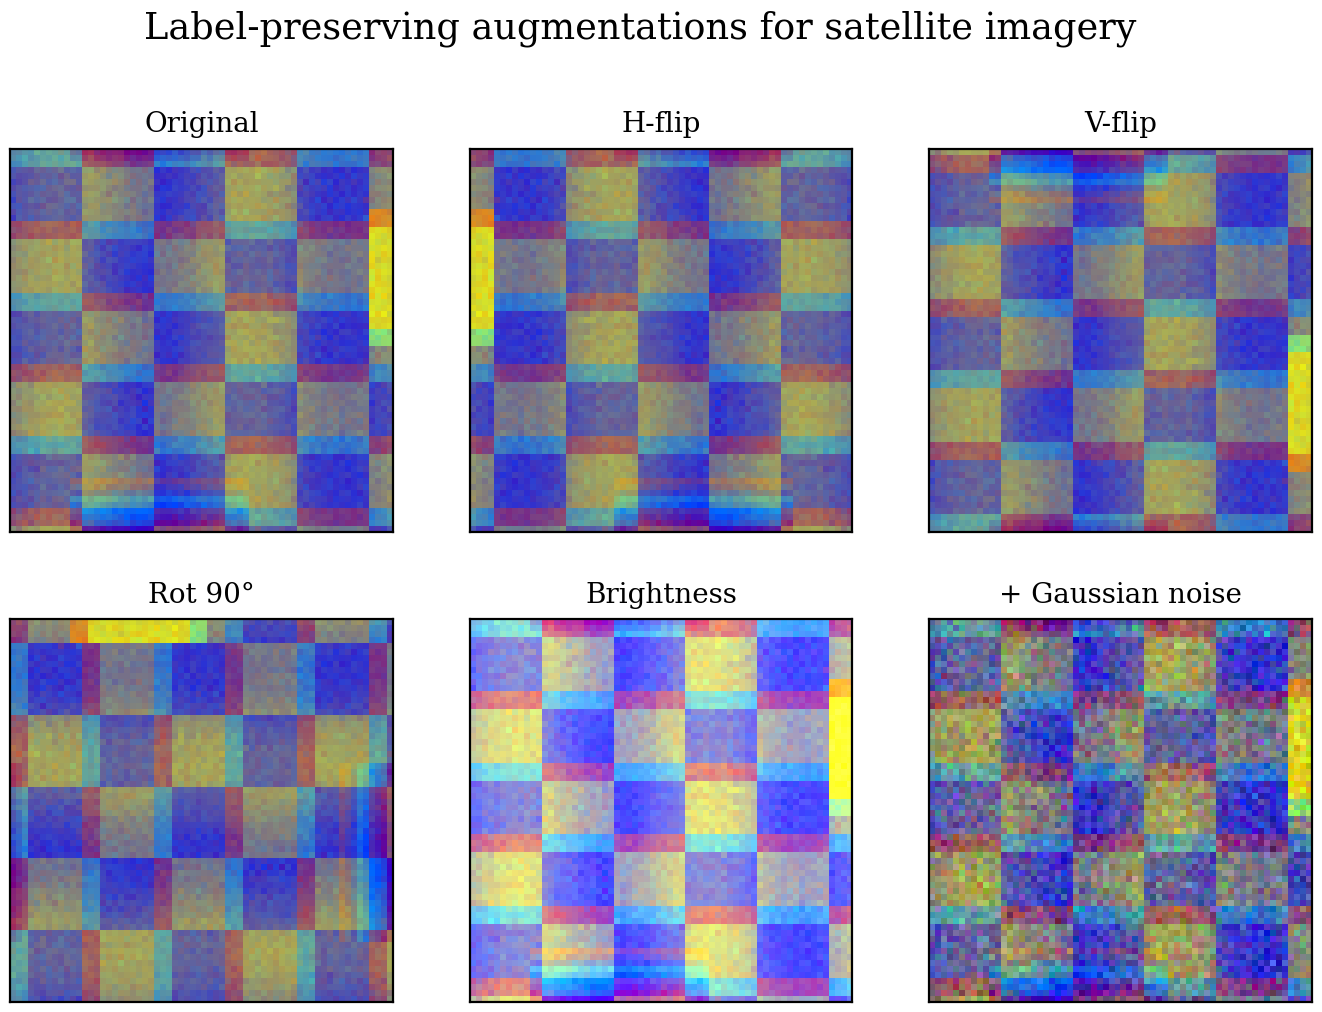
\includegraphics[width=0.86\linewidth]{figures/augmentation.png}
\caption{Label-preserving augmentations. Flips and 90° rotations are exactly
valid for nadir imagery; brightness/contrast jitter and mild Gaussian noise
simulate illumination and sensor variation.}
\label{fig:aug}
\end{figure}

\section{A pipeline with albumentations}

\texttt{albumentations} is fast, supports many bands, and --- crucially for
segmentation --- transforms image and mask jointly. A typical classification
pipeline:
\begin{lstlisting}
import albumentations as A
train_tf = A.Compose([
    A.HorizontalFlip(p=0.5),
    A.VerticalFlip(p=0.5),
    A.RandomRotate90(p=0.5),
    A.RandomBrightnessContrast(0.2, 0.2, p=0.5),
    A.GaussNoise(var_limit=(10, 50), p=0.3),
    A.Normalize(mean=MEAN, std=STD),
])
\end{lstlisting}
Validation/test pipelines contain \emph{only} normalization --- never randomise
the data you measure on.

\paragraph{What to avoid.} Augmentations that break physical meaning hurt EO
models: large hue shifts destroy the spectral signatures that distinguish
materials; heavy elastic/perspective warps fabricate impossible geometry;
aggressive blur erases the texture cues the network relies on. Prefer mild,
physically plausible photometric jitter and rely on the free geometric
invariances.

\section{Joint image--mask augmentation}

For segmentation, every geometric transform applied to the image \emph{must} be
applied identically to the label mask; photometric transforms apply to the image
only. \texttt{albumentations} handles this when you pass both:
\begin{lstlisting}
aug = A.Compose([A.HorizontalFlip(p=0.5), A.RandomRotate90(p=0.5),
                 A.RandomBrightnessContrast(p=0.5)])
out = aug(image=img, mask=mask)          # geometric ops applied to both
img_a, mask_a = out["image"], out["mask"]
\end{lstlisting}
Use nearest-neighbour interpolation for masks (labels are categorical, never
interpolate class indices) and bilinear for images.

\section{MixUp and CutMix}

These mix \emph{pairs} of examples and their labels, regularising decision
boundaries. \emph{MixUp} blends two samples linearly:
\begin{equation}
\tilde{x} = \lambda x_i + (1-\lambda) x_j, \qquad
\tilde{y} = \lambda y_i + (1-\lambda) y_j, \qquad \lambda\sim\mathrm{Beta}(\alpha,\alpha).
\end{equation}
\emph{CutMix} instead pastes a rectangular patch of one image into another and
sets the label mixing coefficient to the patch's area fraction. Both improve
calibration and robustness for classification; for segmentation, CutMix-style
region pasting is more natural than pixel blending. Use them as a complement to,
not a replacement for, geometric augmentation.

\section{Proving it works: an ablation}

Augmentation's value should be measured, not assumed. Train the same model for a
few epochs under increasing augmentation (none $\to$ geometric $\to$
geometric+photometric $\to$ +MixUp) and plot validation accuracy/mIoU. On EO
data the geometric step alone typically yields a clear gain, and the gain grows
as the labelled set shrinks --- the same low-data story as transfer learning.

\begin{keybox}
\begin{itemize}[leftmargin=1.2em,nosep]
  \item Nadir imagery $\Rightarrow$ flips + 90° rotations are exactly label-preserving (8 free views).
  \item Only normalize at validation/test time; never randomise evaluation data.
  \item Avoid hue shifts/heavy warps/blur that destroy spectral or texture cues.
  \item Segmentation: apply geometric ops to image \emph{and} mask (nearest-neighbour for masks).
  \item MixUp/CutMix mix samples and labels; complement geometric augmentation.
\end{itemize}
\end{keybox}

\begin{practbox}
Notebook: \nbpath{chapter\_08\_augmentation/08\_practical\_augmentation\_pipeline.ipynb}.
\begin{enumerate}[leftmargin=1.4em,nosep]
  \item Showcase each transform on one EuroSAT image in a grid.
  \item Build an EO-aware \texttt{albumentations} pipeline; visualise eight random
  draws of one patch.
  \item Demonstrate joint image+mask augmentation on a LoveDA sample.
  \item Implement MixUp and visualise a blended pair with its soft label.
  \item Run a 3-epoch ablation (no-aug vs aug) and plot the accuracy gain.
\end{enumerate}
\end{practbox}

\begin{exbox}
\textbf{8.1 Policy search.} Grid over augmentation strengths; find the policy
maximising validation accuracy without underfitting.\\[2pt]
\textbf{8.2 Custom EO transform.} Implement a band-wise reflectance-jitter
transform that perturbs each band independently within physical bounds.\\[2pt]
\textbf{8.3 Mask safety.} Construct a case where bilinear mask interpolation
creates invalid class indices; fix it with nearest-neighbour.\\[2pt]
\textbf{Mini-project.} Build \texttt{get\_train\_transforms(task, bands)} returning
classification and segmentation pipelines (RGB and multispectral variants) and
document each choice.
\end{exbox}
